% *********************************************************************
% © 2021–2024 Jeremy Sylvestre
%
% Permission is granted to copy, distribute and/or modify this document
% under the terms of the GNU Free Documentation License, Version 1.3 or
% any later version published by the Free Software Foundation; with no
% Invariant Sections, no Front-Cover Texts, and no Back-Cover Texts. A
% copy of the license is included in the appendix entitled “GNU Free
% Documentation License” that appears in the output document of this
% PreTeXt source code. All trademarks™ are the registered® marks of
% their respective owners.
%
% *********************************************************************

\newcommand*{\xmin}{0.5}
\newcommand*{\xmax}{6}
\newcommand*{\ymin}{-5}
\newcommand*{\ymax}{5}
\newcommand*{\func}{\x * \x * \x - 9 * \x * \x + 23 * \x - 14}

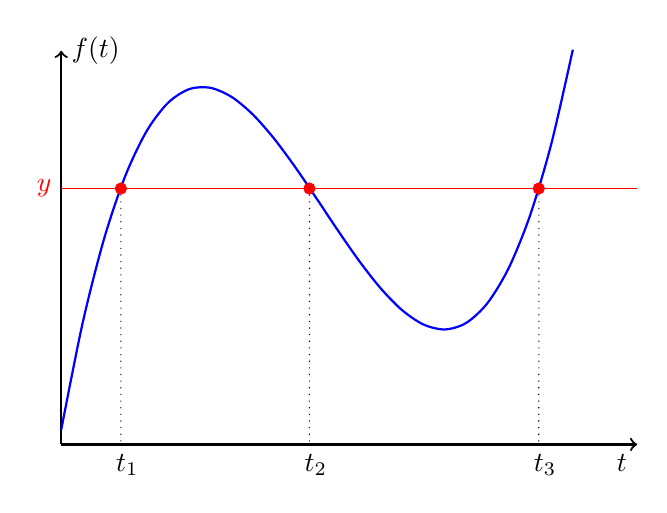
\begin{tikzpicture}
[
	closedpt/.style={circle,draw,fill,inner sep=0pt,minimum size=4pt},
	openpt/.style={circle,draw,inner sep=0pt,minimum size=4pt},
	xscale=1.33,
	yscale=0.5
]

	% \draw[dashed] (1.5,3.625) -- (1.5,\ymin) node[below] {$a$};
	% \draw[dashed] (5.25,3.391) to (5.25,\ymin) node[below] {$b$};

	% axes
	\draw[->,thick] (\xmin,\ymin) -- (\xmax,\ymin) node[below left] {$t$};
	\draw[->,thick] (0.5,\ymin) -- (0.5,\ymax) node[right] {$f(t)$};

	\draw[red] (\xmax,1.5) -- (\xmin,1.5) node[left] {$y$};

	% example graph
	\draw[thick, domain=0.5:5.385, smooth, blue] plot (\x,{\func});

	\node[closedpt,red] at (1.07,1.5) (pt) {};
	\draw[dotted] (pt) -- (1.07,\ymin) node[below,xshift=0.08cm] {$t_1$};
	\node[closedpt,red] at (2.87,1.5) (pt) {};
	\draw[dotted] (pt) -- (2.87,\ymin) node[below,xshift=0.08cm] {$t_2$};
	\node[closedpt,red] at (5.06,1.5) (pt) {};
	\draw[dotted] (pt) -- (5.06,\ymin) node[below,xshift=0.08cm] {$t_3$};

\end{tikzpicture}
